<<<<<<< HEAD
=======
\documentclass{theme_cnrs}
\usepackage[absolute,overlay]{textpos}
\usepackage{graphicx}
\title{}
\author{Aghilas SINI}
\date{}
\institute{LORIA UMR 7503}



%% package for tikz
\usepackage{tikz}
\usetikzlibrary{shapes,arrows}
\usepackage{amsmath,bm,times}
\usetikzlibrary{shapes,snakes,arrows,shadows}
\usetikzlibrary{matrix}
\usetikzlibrary{shapes.geometric}
\usetikzlibrary{positioning}
\usepackage{subcaption}

\setbeamercovered{transparent} 
%animation
\tikzset{
  invisible/.style={opacity=0.2},
  visible on/.style={alt={#1{}{invisible}}},
  alt/.code args={<#1>#2#3}{%
    \alt<#1>{\pgfkeysalso{#2}}{\pgfkeysalso{#3}} % \pgfkeysalso doesn't change the path
  },
}


%
\newcommand{\mx}[1]{\mathbf{\bm{#1}}} % Matrix command
\newcommand{\vc}[1]{\mathbf{\bm{#1}}} % Vector command

% We need layers to draw the block diagram
\pgfdeclarelayer{background}
\pgfdeclarelayer{foreground}
\pgfsetlayers{background,main,foreground}

% Define a few styles and constants
\tikzstyle{sensor}=[draw, fill=blue!20,rounded corners, text width=5em, 
    text centered, minimum height=2.5em]
\tikzstyle{block}=[sensor,visible on=<#1->]

\tikzstyle{input}=[fill=blue!20, regular polygon, regular polygon sides=3,rotate=-90,visible on=<#1->]
\tikzstyle{ann} = [above, text width=5em,visible on=<#1->]
\tikzstyle{naveqs} = [sensor, text width=6em, fill=black!20, 
    minimum height=12em, rounded corners,visible on=<#1->]
\tikzstyle{psola} = [sensor, text width=4em, fill=green!40, 
    minimum height=10em, rounded corners,visible on=<#1->]


\def\blockdist{4.3}
\def\edgedist{1.2}
%%







\begin{document}

{
        \usebackgroundtemplate{
\includegraphics[width=\paperwidth]{theme_cnrs_logo_white.png}}
       % \usebackgroundtemplate{
\includegraphics[width=\paperwidth]{theme_cnrs_logo_light-blue.png}}
        \frame[plain]{
               \titlepage
        }
}



%%%%%%%%%%%%%%%%%%%%%%%%%%%%%%%%%%%%%%%%%%%%%%%%%%%%%%%%%%%%%%%%%%%%%%%%%%%%%%%%%%%
%% IFCASL Project
%%%%%%%%%%%%%%%%%%%%%%%%%%%%%%%%%%%%%%%%%%%%%%%%%%%%%%%%%%%%%%%%%%%%%%%%%%%%%%%%%%%

\frame{
 \frametitle{IFCASL project}
\begin{itemize}
	\item Department of Computational Linguistics and Phonetics, university of saarbrücken, Germany.
	\item Multispeech Team, LORIA\--INRIA, France
	\item Topics Language Learning.
\end{itemize}
\begin{textblock*}{10cm}(4.5cm,7cm) % {block width} (coords)

\includegraphics[width=1.75cm]{Logo_LORIA.jpeg}
\end{textblock*}
\begin{textblock*}{10cm}(6.5cm,7cm) % {block width} (coords)

\includegraphics[width=1.75cm]{logo_uds.png}
\end{textblock*}
}


\frame{
       \frametitle{IFCASL project}
       \section*{CAPT  Computational Assisted Pronunciation Training}
       \begin{itemize}
              \item Speech recognition $\rightarrow $ Speech Text Alignment
              \item Scoring $\rightarrow$ Score of the result of the
              \item Error Detection $\rightarrow$ Example Fricative / Occlusive Mispronounced
              \item Error Diagnosis $\rightarrow$ Automatic Diagnosis of the Above Error For Example
              \item Feedback presentation $\rightarrow$ Audio Feedback (Give Correction: Modifier the Learner Signal ) 
              
       \end{itemize}
}

\frame{

\frametitle{IFCASL project}

}


%%%%%%%%%%%%%%%%%%%%%%%%%%%%%%%%%%%%%%%%%%%%%%%%%%%%%%%%%%%%%%%%%%%%%%%%%%%%%%%%%%%
%% ORTOLANG Project
%%%%%%%%%%%%%%%%%%%%%%%%%%%%%%%%%%%%%%%%%%%%%%%%%%%%%%%%%%%%%%%%%%%%%%%%%%%%%%%%%%%
\frame{
\frametitle{ORTOLANG project }

\begin{itemize}
\item Involved Teams Synalp and Multispeech.
\item Topics Speech Recognition, Natural Language Processing
\item Speech Toolkit CMU Sphinx
\end{itemize}


\begin{textblock*}{10cm}(1cm,7cm) % {block width} (coords)

\includegraphics[width=2cm]{Logo_ATILF_new.png}
\end{textblock*}
\begin{textblock*}{10cm}(3.5cm,7cm) % {block width} (coords)

\includegraphics[width=1.75cm]{Logo_LORIA.jpeg}
\end{textblock*}
\begin{textblock*}{10cm}(5.5cm,7cm) % {block width} (coords)

\includegraphics[width=1.75cm]{INRIA_CORPO_RVB.jpg}
\end{textblock*}

\begin{textblock*}{10cm}(7.5cm,6.5cm) % {block width} (coords)

\includegraphics[width=1.75cm]{mariane-avenir.png}
\end{textblock*}
\begin{textblock*}{10cm}(9.5cm,6.75cm) % {block width} (coords)

\includegraphics[width=3.0cm]{logo-Universite-de-Lorraine.jpg}
\end{textblock*}

}
\frame{
\frametitle{ORTOLANG Project}


}



%%%%%%%%%%%%%%%%%%%%%%%%%%%%%%%%%%%%%%%%%%%%%%%%%%%%%%%%%%%%%%%%%%%%%%%%%%%%%%%%%%%
%% Speech Synthesis Pipeline
%%%%%%%%%%%%%%%%%%%%%%%%%%%%%%%%%%%%%%%%%%%%%%%%%%%%%%%%%%%%%%%%%%%%%%%%%%%%%%%%%%%
\frame{


\frametitle{ Speech Synthesis Pipeline}
\begin{figure}

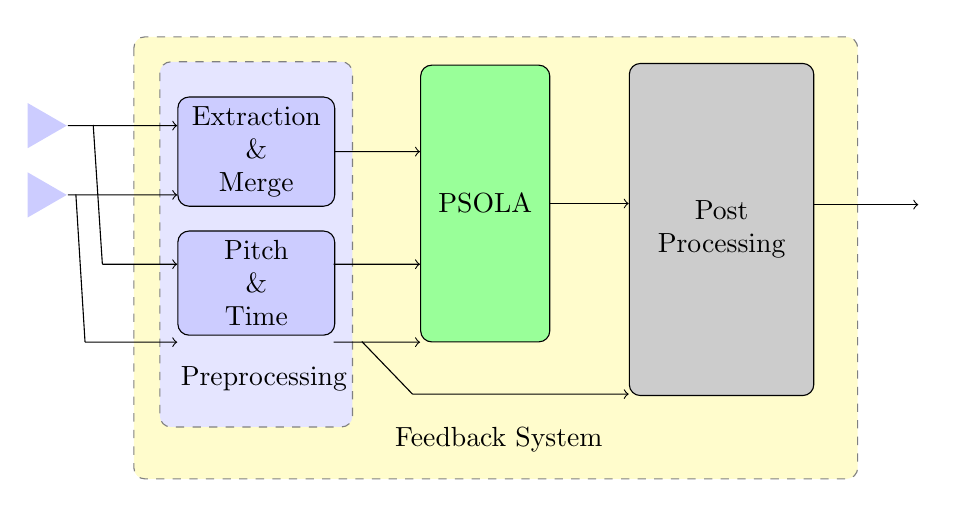
\begin{tikzpicture}[scale=1.1]
    \node (naveq) [naveqs={1}] {Post \\ Processing};
     	
 	\path (naveq.0)+(-3.8,+0.3) node (psola) [psola={1}] {PSOLA};
      
    \path (naveq.140)+(-\blockdist,0) node (gyros) [block={1}] {Extraction \\ \& \\ Merge};
    \path (naveq.-150)+(-\blockdist,0) node (accel) [block={1}] {Pitch \\ \& \\ Time };
	\path (gyros.0)+(-3.4,+0.3) node (teacher) [input={1}] {};
    \path (gyros.0)+(-3.4,-0.5) node (learner) [input={1}] {};
 	
\path [draw, ->] (teacher) -- node [above] {} 
        (gyros.west |- teacher);
\path [draw, ->] (learner) -- node [above] {} 
        (gyros.west |- learner);
%\draw[<-] (accel.west) -- +(-0.8,0);
%\draw[<-] (accel.west) -- +(-0.8,0	);
\path (gyros.0)+(-2.8,-1.30) node (ref1){}; 
\path (gyros.0)+(-3.0,-2.2) node (ref2){};
%
\path (gyros.0)+(-2.8,+0.42) node (refTeacher){}; 
\path (gyros.0)+(-3.0,-0.38) node (refLearner){};
%
\path (gyros.east)+(-0.13,-1.30) node (pitch){}; 
\path (gyros.east)+(-0.13,-2.2) node (time){};
%
\path (gyros.east)+(+0.2,-2.080) node (ref1Pitch){}; 
\path (psola.west)+(-0.2,-2.2) node (ref2Pitch){}; 
\path [draw, ->] (ref1) -- node [above] {} 
        (accel.west |- ref1);
 
\path [draw, ->] (ref2) -- node [above] {} 
        (accel.west |- ref2);

\path [draw, ->] (gyros) -- node [above] {} 
        (psola.west |- gyros);

\path [draw, -] (refTeacher)--(ref1.east);

\path [draw, -] (refLearner) -- (ref2.east);

\path [draw, ->] (pitch) -- node [above] {} 
        (psola.west |- pitch);

\path [draw, ->] (time) -- node [above] {} 
        (psola.west |- time);

\path [draw, ->] (ref2Pitch) -- node [above] {} 
        (naveq.west |- ref2Pitch);

\path [draw, -] (ref1Pitch) -- (ref2Pitch.east);

\path [draw, ->] (psola.east) -- node [above] {} 
        (naveq.west |- psola.east);
    \path (accel.south west)+(+1.0,-0.5) node (IMU) {Preprocessing};
    \path (naveq.south west)+(-1.5,-0.5) node (INS) {Feedback System};
    \draw [->] (naveq.15	) -- node [ann={1}] {} + (\edgedist,0) 
        node[right] {};
 
    \begin{pgfonlayer}{background}
        % Compute a few helper coordinates
        \path (gyros.west |- naveq.north)+(-0.5,0.3) node (a) {};
        \path (INS.south -| naveq.east)+(+0.5,-0.2) node (b) {};
        \path[fill=yellow!20,rounded corners, draw=black!50, dashed]
            (a) rectangle (b);
        \path (gyros.north west)+(-0.2,0.4) node (a) {};
        \path (IMU.south -| gyros.east)+(+0.2,-0.3) node (b) {};
        \path[fill=blue!10,rounded corners, draw=black!50, dashed]
            (a) rectangle (b);
    \end{pgfonlayer}
\end{tikzpicture}
\caption{Schema Block of Feedback Correction System }
\end{figure}


}

\frame{
\frametitle{My Master }	


}






\end{document}
>>>>>>> 81132a7c26c7db5853ecdd6375f4041b5b8d685e
